\documentclass[12pt,t]{beamer}
\usepackage{pslatex}
\usepackage[T1]{fontenc}       
\usepackage[utf8]{inputenc}    % pour les accents (mettre latin1 pour windows au lieu de utf8)
\usepackage[frenchb]{babel}
\usepackage{amsmath,amsfonts,amsthm} % Math packages

\usetheme[nat, TPlrimage = "ImgDLinks.JPG", logostyle=none,
headstyle=institute]{Frederiksberg}

\usepackage{colortbl}
\definecolor{bg}{RGB}{235,235,235}
\definecolor{bk}{RGB}{135,135,135}
\newcommand{\class}[1]{\colorbox{bg}
{\textcolor{red}{\usefont{OT1}{cmtt}{m}{n}#1}}}

\title{Liens dansants}
\subtitle{Algorithme X et ses applications}
\author{Zhixing CAO, Yuxiang LI}
\institute{INF\ 441}
\date[]{\today}

% If you wish to uncover everything in a step-wise fashion, uncomment
% the following command:

%\beamerdefaultoverlayspecification{<+->}

\begin{document}

\frame[plain]{\titlepage}

\section{Introduction}

\begin{frame}
\frametitle{Plan}
\tableofcontents[currentsection]
\end{frame}

\begin{frame}
\frametitle{Liens dansants} 
Réinserer x dans la liste en temps constant
\begin{center}
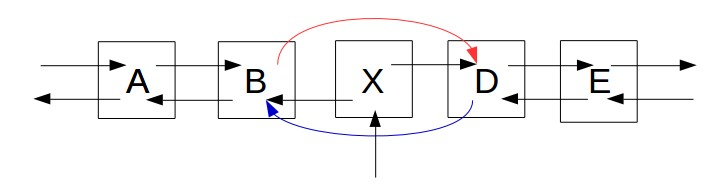
\includegraphics[width=.95\textwidth]{noeud.jpg}
\label{fig:node}
\end{center}
\end{frame}

\begin{frame}
\frametitle{EMC et Algorithme X}
\begin{center}
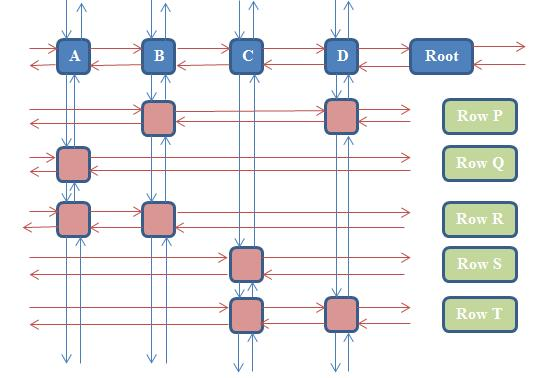
\includegraphics[width=.85\textwidth]{ImgDLinks.JPG}
\label{fig:dlx}
\end{center}
\end{frame}

\section{Organisation du code}

\begin{frame}
\frametitle{Plan}
\tableofcontents[currentsection]
\end{frame}

\begin{frame}
\frametitle{Structure}
\begin{center}
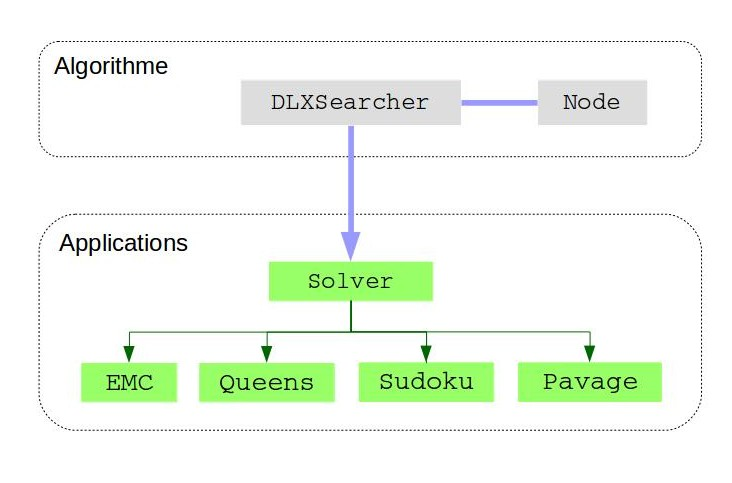
\includegraphics[width=1.0\textwidth]{structure.jpg}
\label{fig:structure}
\end{center}
\end{frame} 

\section{Applications}

\begin{frame}
\frametitle{Plan}
\tableofcontents[currentsection]
\end{frame}

\begin{frame}
\frametitle{EMC généralisé}
Colonnes secondaires : une relaxation
\begin{itemize}
  \item Compter les colonnes sautées
  \item Sauter une colonne tant qu'il y a la possibilité
\end{itemize}
\begin{center}
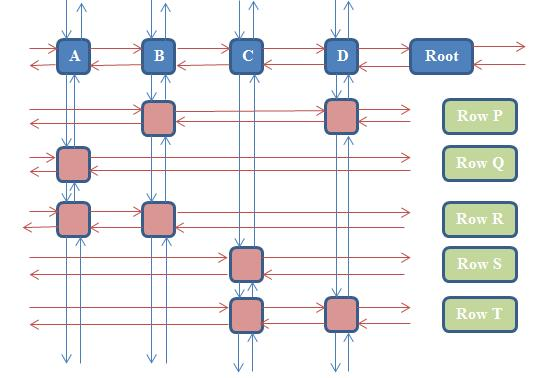
\includegraphics[width=.65\textwidth]{ImgDLinks.JPG}
\label{fig:dlxx}
\end{center}
\end{frame}

\begin{frame}
\frametitle{N-Reines}
\begin{itemize}
  \item Colonnes : $N$ rangs, $N$ colonnes et $4N - 2$ diagonaux
  \item Rang : $N \times N$ positions
\end{itemize}
\begin{center}
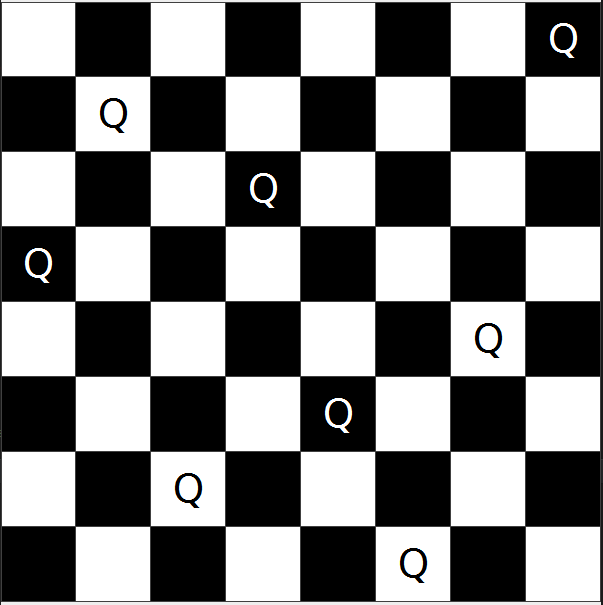
\includegraphics[width=.5\textwidth]{queens.png}
\label{fig:queens}
\end{center}
\end{frame}

\begin{frame}
\frametitle{Sudoku}
\begin{itemize}
  \item Colonnes : $N^2$ positions, $N \times 3N$ pour les détails
  \item Rang : $N^2$ positions avec $N$ nombres chacune
\end{itemize}
\begin{center}
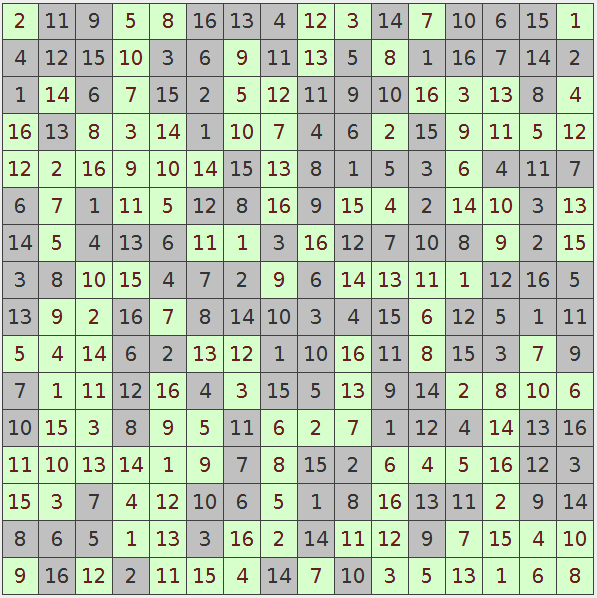
\includegraphics[width=.5\textwidth]{sudoku.png}
\label{fig:sudoku}
\end{center}
\end{frame}

\begin{frame}
\frametitle{Pavage}
\begin{itemize}
  \item Colonnes : $M$ types, $N$ cases à occuper
  \item Rang : à calculer
\end{itemize}
\begin{center}
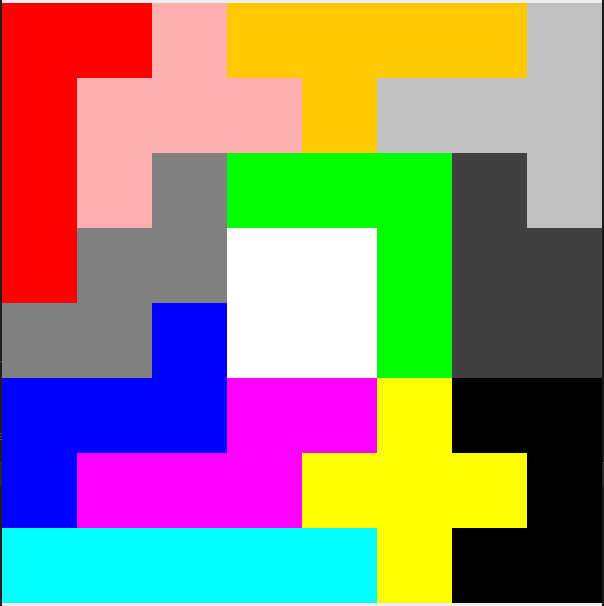
\includegraphics[width=.5\textwidth]{pavage.png}
\label{fig:pavage}
\end{center}
\end{frame}

\section{Analyse du résultat}

\begin{frame}
\frametitle{Plan}
\tableofcontents[currentsection]
\end{frame}

\begin{frame}
\frametitle{Analyse du résultat}
La complexité dépend de : 
\begin{itemize}
  \item Taille de la matrice
  \item Densité de la matrice
  \item Nombre de solutions
  \item \ldots
\end{itemize}
Les avantages de l'algorithme X :
\begin{itemize}
  \item Réduire l'arbre de recherche
  \item Simplifier l'étape de vérification
  \item \ldots
\end{itemize}
\end{frame}

\section{Démonstration}

\begin{frame}
\frametitle{Plan}
\tableofcontents[currentsection]
\end{frame}

\end{document}
